\documentclass{bioinfo}
\usepackage{url}
\copyrightyear{2014}
\pubyear{2014}

\def\Put(#1,#2)#3{\leavevmode\makebox(0,0){\put(#1,#2){#3}}}
\begin{document}
\firstpage{1}

\title[Homology-based function prediction]{HypfuNN -- Homology-based protein function prediction using neural networks}
\author[]{Jonathan Boidol\,$^{1}$, Rene Schoeffel\,$^{1}$ and Yann Sp\"ori\,$^{1}$}
\address{$^{1}$TUM (Technische Universit\"at M\"unchen) Department of Informatics, Bioinformatics \& Computational Biology - i12, Boltzmannstr.~3, 85748 Garching/Munich, Germany}
\history{}

\editor{}

\maketitle

\begin{abstract}

\section{Motivation:} 
Faced with a huge gap in the number of available sequences and available functional annotations, the prediction of protein function helps to identify research targets, understand diseases and close gaps in our knowledge of molecular processes. We use the available annotation data to transfer function descriptions to proteins with known sequence but unknown function (the standard case in public databases) from functionally characterized homologs. 
\section{Results:}
We identify homologs via blast and hhblits search in a database of annotated proteins and feed the annotations from these proteins to a neural network that assesses the confidence of a transfer and finetunes our prediction. To circumvent the difficulties of functional annotations in human language, we restrict annotations in training and prediction to terms from the human phenotype ontology (HPO). In a crossvalidation on a set of 2815 HPO-annotated proteins, we achieve an F-max measure of $0.xx \pm xx$. We also provide HPO annotations for the complete human proteome.

\section{Availability:} The datasets, predictor and predictions are available upon request.

\section{Contact:} \href{boidolj@in.tum.de}{boidolj@in.tum.de}, \href{spoeri@in.tum.de}{spoeri@in.tum.de}, \href{schoeffel@in.tum.de}{schoeffel@in.tum.de}
\end{abstract}

\section{Introduction}

Overwhelmed with genomic data, biologists are facing a wealth of easily accessible sequence data but there is little use in this data without verified experimental annotation. Especially interesting, but also difficult to obtain and consequently sparse is the functional annotation of proteins, which helps to understand life at the molecular level and is e.g.~important in understanding and curing diseases. Homology-based function prediction fills the gap by transferring verified annotations to related proteins of unknown function under the reasonable assumption that function is at least partly conserved between homologs -- homologs to a kinase will likely still function as kinases but  with different substrates. A generic procedure is shown in figure \ref{fig:function_transfer}. We implemented such a homology-based approach with HypfuNN, our Homology-based protein function predictor utilizing neural networks. This working paper first describes details of the implementation, then presents the results of a 10 times 10-fold crossvalidation on a dataset of 2,815 protein sequences annotated with the HPO ontology of human phenotypes~\citep{Koehler2014} collected from public databases.

\begin{figure}[!hb]
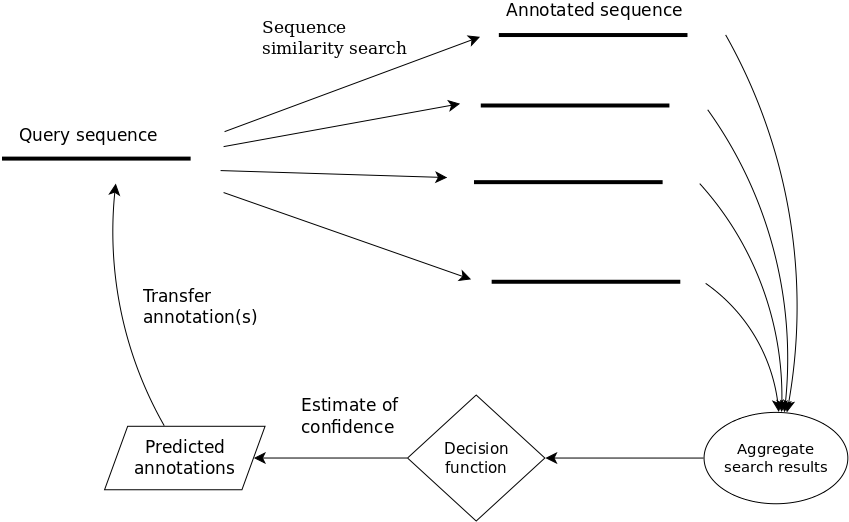
\includegraphics[width = 0.4\textwidth]{figures/function_transfer.png}
\caption{Homologs to a query sequence can be detected via similarity search, e.g.~blast, and annotations transferred back to the query sequence.}
\label{fig:function_transfer}
\end{figure}


\begin{methods}
\section{Methods}

\subsection{Dataset}

HypfuNN was developed as CAFA~\citep{CAFA} entry competing against function prediction methods by other student groups. In order to compare the fitness of the implemented prediction methods, a common
dataset for training and testing for all groups was used, as described in the implementation part. The dataset contains 2815 HPO-annotated proteins.

\subsection{Implementation}

As already described above, we predict protein annotations by homology. Proteins, that have the same function, so called homologs, tend to share a similar sequence. In order to identify proteins
with similar sequence, we are using blast and hhblits. For both, blast and hhblits, we require an minimal e-value of 1, to exclude weak similar protein sequences. Our tool supports to use
different blast e-value with the commandline option -e, as well as looking up similar proteins in other databases with the commandline options -b for blast and -l for hhblits.\newline
In order to map the annotations of the found proteins to the query sequence, our tool is looking up the annotations for each found similar sequence hit. This step is done by an identifier hpo terms mapping
file. Our method support the use of different mapping files with the commandline option -c.\newline
Since hpo is a hierarchical annotation system, each found annotation represent a tree. In order to merge these annotation trees, each node of each tree is annotated with information about the sequence
hit. Hereby our method supports the fact, that some hpoterms have more than a single parent node.\newline
\begin{figure}[!hb]
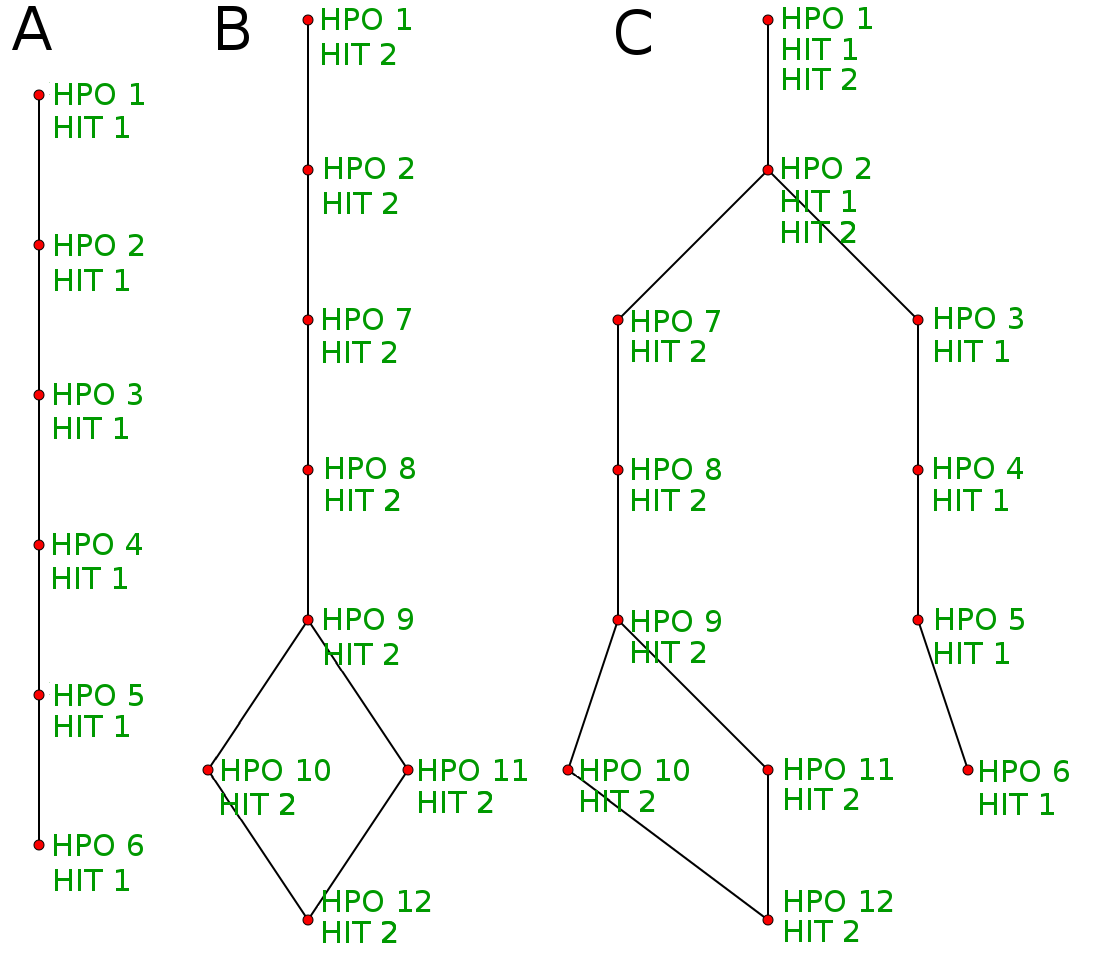
\includegraphics[width = 0.4\textwidth]{figures/merge_trees.png}
\caption{Merge trees TODO}
\label{fig:function_transfer}
\end{figure}
In order to predict whether a single annotation node can be transfered to the query sequence, we merge the found subtrees together (Figure \ref{fig:function_transfer}). By default, for the tree merging,
all subtrees are taken into account. However when calling our method with the commandline option --fast, only the annotation trees for the best 6 hits (by e-value) will be merged.\newline
Using the pyBrain\footnote{citation} toolkit, we trained a neuronal network, to find annotation nodes that may be transfered to the query sequence. For this step, the following features were taken into
account:
\begin{itemize}
\item the length of the query sequence
\item number of hits
\item longest hit
\item avg hit
\item min E-Val
\item avg E-Val
\item product of E-Val
\item best e-value from blast or hhblits
\item min heigth of HPO-Tree
\item max heigth in HPO-Tree
\item max. overlap of query and all hits
\item length of best hit
\end{itemize}
The used neuronal network has an input node for each of the above mentioned features, as well as two hidden layers. The first hidden layer contains features + 1 nodes, while the second hidden layer
contains 3 nodes. The first output node predict whether we may transfer the given annotation to the query sequence. The second output node predicts whether we may not transfer the annotation.
The difference between the two output nodes is taken as the methods confidence.


\end{methods}
\section{Results and Discussion}

\subsection*{F-measure and ROC-curve}
In a 10 times 10-fold crossvalidation, our predictor achieves an average F-max (the highest F-measure for any given confidence level) of $0.35\pm 0.03$ at a confidence level of $0.34$. Figure \ref{img:preRec_ROC} shows the precision recall and ROC curves averaged over the tenfolds of the crossvalidation. The sharp jumps in both curves are an artefact of jumps in the confidence function that clusters around few values for most predictions. In future releases of HypfuNN we hope to achieve a smoother confidence score with optimized activation functions in the output layer of the neural network.

\begin{figure}[!h]
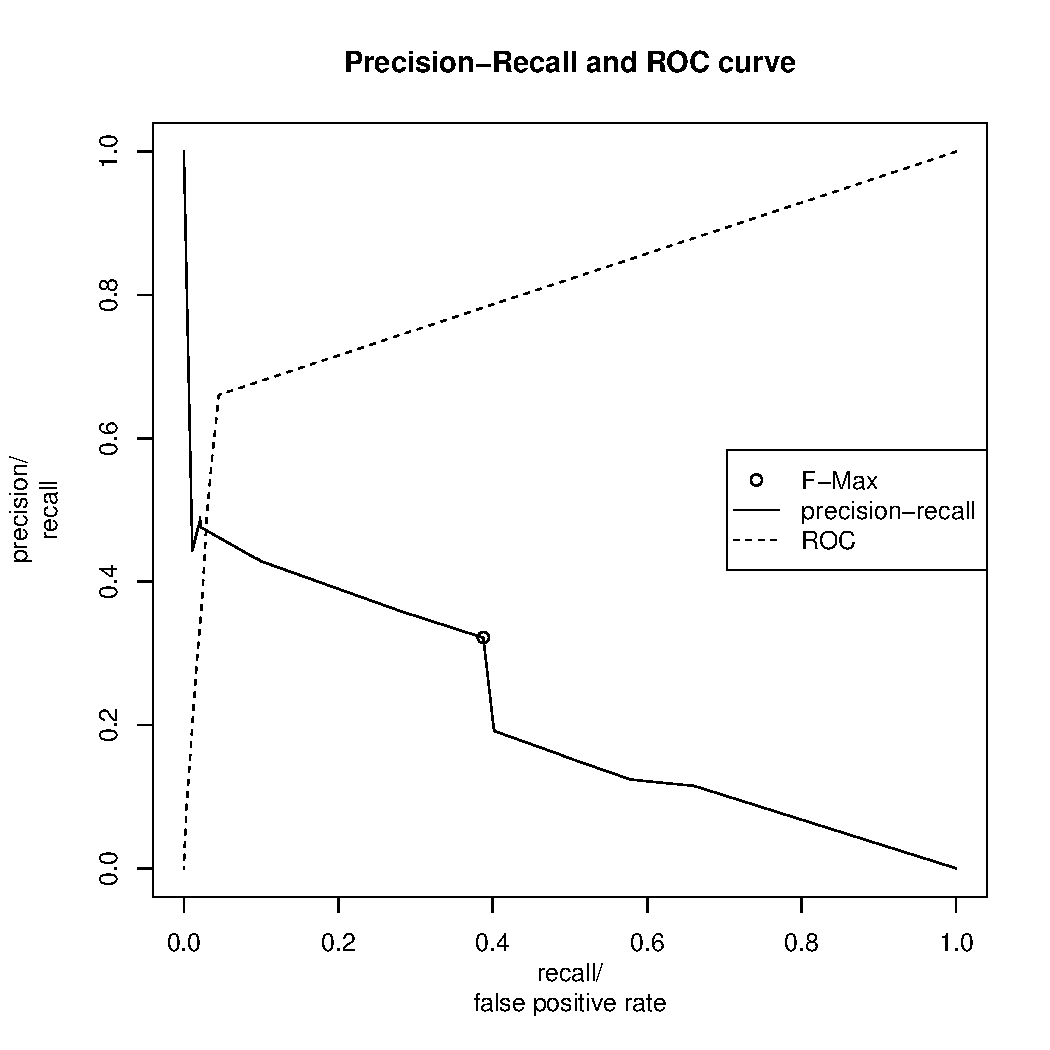
\includegraphics[width=0.45\textwidth]{figures/PreRecROC.pdf}
\caption{Precision-Recall curve (solid line) of HypfuNN predictions. The best F-measure is achieved at confidence $0.34$ with precision $0.32 \pm 0.04$ and recall $0.39 \pm 0.10$. The second set of axes and dashed line describe the ROC curve of HpyfuNN predictions.}
\label{img:preRec_ROC}
\end{figure}

\subsection*{Predictions for Human Proteome}

For 20231 human protein sequences provided the CAFA challenge, our predictor provides 3.9 mio HPO-terms with a confidence larger than $0.34$, the threshold for our F-max value. These predictions are reduced to the most specific terms with equal confidence, i.e.~a parent node that is predicted with an equal confidence as a child, it is not counted separately. Assuming our error measures hold in general, we add 1.2 mio correct functional annotations to largely not yet described protein sequences. On the flipside, we also add many false annotations, although it can be expected that some of them lead in the right direction. For example if we incorrectly predict a HPO term, but the parent of this term is correct, then our prediction is strictly counted only as false positive, but still could give a valuable lead to the proteins correct function.

\section{Conclusion}


Homology based prediction is a standard technique in the bioinformatics community. Our predictor uses the hierarchical structure of the Human Phenotype Ontology to aggregate available information from different levels of the hierarchy. We try to improve over simple sequence similarity measures with a neural network designed to improve our functional predictions and add a measurable confidence to each prediction. Future research will hopefully be concentrated on optimizing the feature set and network architecture to improve training speed and prediction accuracy. We hope that our presented approach helps to understand and explore the possibilities and challenges that lie in the prediction of functional annotations.

\section*{Acknowledgement}
We thank all the organizers of the lecture protein prediction 2, especially Lothar Richter, for guiding all groups through this project with useful comments. Also thanks to Prof.~Rost for his insightful
comments.
%\paragraph{Conflict of interest\textcolon} none declared

\bibliographystyle{bioinformatics}
\bibliography{references}

\end{document}
